\documentclass[12pt,letterpaper]{article}
\usepackage{fullpage}
\usepackage{ctex}
\usepackage{algorithm}
\usepackage{algorithmic}
\usepackage[top=2cm, bottom=4.5cm, left=2.5cm, right=2.5cm]{geometry}
\usepackage{amsmath,amsthm,amsfonts,amssymb,amscd}
\usepackage{lastpage}
\usepackage{enumerate}
\usepackage{fancyhdr}
\usepackage{mathrsfs}
\usepackage{xcolor}
\usepackage{graphicx}
\usepackage{listings}
\usepackage{hyperref}

\hypersetup{%
  colorlinks=true,
  linkcolor=blue,
  linkbordercolor={0 0 1}
}
 
\renewcommand\lstlistingname{Algorithm}
\renewcommand\lstlistlistingname{Algorithms}
\def\lstlistingautorefname{Alg.}

\lstdefinestyle{Python}{
    language        = Python,
    frame           = lines, 
    basicstyle      = \footnotesize,
    keywordstyle    = \color{blue},
    stringstyle     = \color{green},
    commentstyle    = \color{red}\ttfamily
}

\setlength{\parindent}{0.0in}
\setlength{\parskip}{0.05in}

% Edit these as appropriate
% \newcommand\hwnumber{1}                  % <-- homework number
\newcommand\NetIDa{1801110566}           % <-- NetID of person #1
%\newcommand\NetIDb{netid12038}           % <-- NetID of person #2 (Comment this line out for problem sets)

\pagestyle{fancyplain}
\headheight 35pt
\lhead{\NetIDa}
\lhead{\NetIDa\\修格致}                 % <-- Comment this line out for problem sets (make sure you are person #1)
\chead{\textbf{\Large Phase Transition}}
\rhead{bigdata \\ \today}
\lfoot{}
\cfoot{}
\rfoot{\small\thepage}
\headsep 1.5em

\begin{document}

\section*{问题描述}

这次应该不会自动编译了吧。。。

我们要实现下面两个算法之一。

\subsection*{LinearTimeSVD算法}

线性时间SVD算法的策略是:选取矩阵$A$的$c$列,每列重新标注,形成一个新矩阵$C\in\mathbb{R}_{m\times c}.$ 然后通过对$C^TC$进行通常的SVD分解,计算$C$的奇异值和左奇异向量。这可以近似$A$的奇异值和左奇异向量。

\begin{figure}[h]
    \centering
    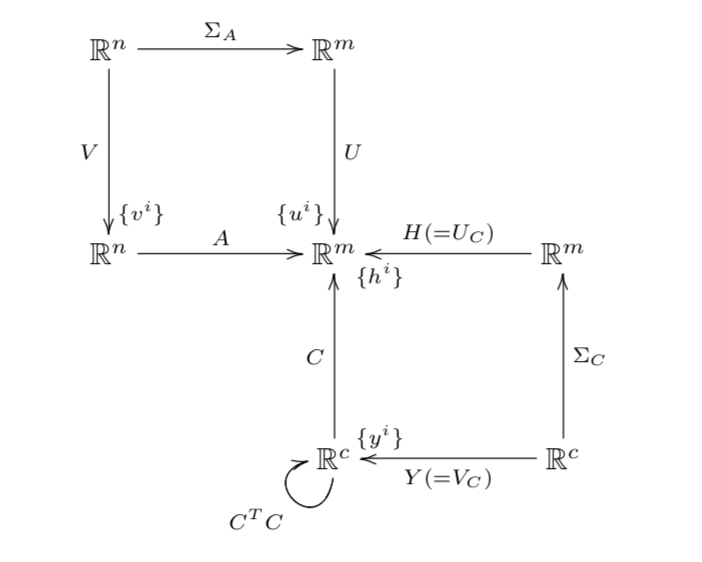
\includegraphics{ltsvd.png}
    \caption{LinearTimeSVD算法}
    \label{ltsvd}
\end{figure}

图片\ref{ltsvd}是该算法的示意图。

\subsection*{Proto-Algorithm: Solving the Fixed-Rank Problem}

第二种算法的思路如下图\ref{pasfrp}所示:

\begin{figure}[h]
    \centering
    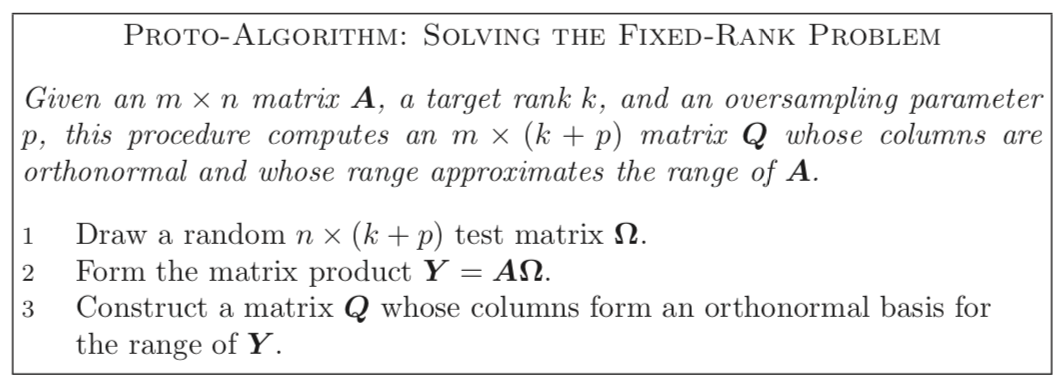
\includegraphics[width = 0.5\textwidth]{randomizedprototype.png}
    \caption{Proto-Algorithm: Solving the Fixed-Rank Problem}
    \label{pasfrp}
\end{figure}

我在这次作业中,选择了第一种算法,用python语言对其进行实现。

\section*{实验}

\subsection*{随机生成数据}

通过下面的设置取得一个矩阵,并求出其前$r\in\{5,10,15,20\}$大的奇异值,以及其奇异向量。

\begin{lstlisting}[language={python}]
    m = 2048
    n = 512
    p = 20
    A = randn(m,p)*randn(p,n)
\end{lstlisting}

得到的结果如下:

\begin{table}[h]
\centering
\begin{tabular}{|l|l|l|l|}
\hline
$r$ & exp1: $t$ & exp2: $t$ & exp3: $t$\\ \hline
 5 &    0.08126497268676758  &  0.06409597396850586   & 0.07390093803405762 \\ \hline
10 &   0.03443193435668945   & 0.025016069412231445 & 0.03003096580505371
\\ \hline
15 & 0.03320908546447754 &   0.035800933837890625  & 0.03665590286254883
  \\ \hline
20 & 0.034197092056274414 & 0.03660106658935547 & 0.040490150451660156 \\ \hline
\end{tabular}
\end{table}

我对$r=\{5,10,15,20\}$进行了3组实验,得到的运行时间如上表所示。可见运行时间较为稳定,可以在线性时间内运行完毕。

\subsection*{rSVD-single-pass数据集}

这个部分里,我复现了\url{https://github.com/WenjianYu/rSVD-single-pass}中生成随机数据集的算法,写在\emph{generatedata.py}文件中。并测试了对于$m = n = 2\times 10^3.$ 的矩阵的计算时间的三次试验结果\footnote{我尝试生成了$2\times 10^5$阶矩阵的数据集,但是内存超了,所以没有呈现在报告上。特此说明。}。

\begin{table}[h]
\centering
\begin{tabular}{|l|l|l|l|}
\hline
r & exp1-timing & exp2-timing & exp3-timing \\ \hline
  50  & 0.4229423999786377 &0.4193081855773926& 0.4090569019317627 \\ \hline
 100  & 0.4109618663787842&0.5056757926940918& 0.4087069034576416\\ \hline
 150  & 0.451876163482666&0.4589710235595703& 0.43385791778564453\\ \hline
 200  & 0.5109848976135254&0.5014669895172119& 0.4837648868560791\\ \hline
 500  & 0.994359016418457&0.9467556476593018& 0.9239499568939209\\ \hline
 1000  & 2.2344188690185547&2.214768886566162& 2.300198793411255\\ \hline
 1500  & 4.6173412799835205& 4.693850994110107& 4.715956926345825\\ \hline
\end{tabular}
\end{table}

可见,运行时间比较稳定,算法是有效的。



\end{document}
